\section{Functionality}
\label{sec:functionality}
%
This chapter describes the terminology and principle of the tool \Tool.


\subsection{System Specification}
\label{sec:inputs}
This section introduces the system model of \Tool.
All systems that fulfill this system model can be analyzed by \Tool.
At the end of the section, some practical examples for such systems are given.


\subsubsection{System Model}
\label{sec:system-model}
To analyze the timing of one or more cause-effect chains, a model of the hardware-software system is required. 
The system model represents the hardware platform and the application software neglecting all aspects that do not determine the timing of the system. 
In the following, the system model for \Tool is specified.
\bigskip

A \emph{hardware platform} $\platform = (\ResourceSet, \linkSet)$ is a directed graph.
A vertex of the graph is an element from the set of resources $\ResourceSet$.
The edges $\linkSet$ correspond to the directed physical connections between resources.
%
A \emph{resource} $\Resource \in \ResourceSet$ is characterized by the property that it provides processing or communication service to tasks according to a given scheduling policy. 
A resource can thus be a processor core, a data bus, etc.  
We assume that the clocks of all resources are perfectly synchronized. 

A \emph{task} $\taskStd \in \taskSet$ is a service-consuming entity. 
This definition is very general and corresponds to the concept of a task in the real-time community.
Since consumed service can be processing service or communication service; we do not need to distinguish between notions like 'software tasks' and 'messages'. 
The $j$th instance of a task $\taskStd$ is called job $\jobStd$.
Two variants of a task exist (see also Figure \ref{fig:task}): 
\bigskip

%\begin{tcolorbox}[colback=black!5!white,colframe=black!75!black, breakable, title= Bounded execution time (BET) task]
\begin{definition}[Bounded execution time task]
The bounded execution time (BET) task is characterized by the following attributes
	\begin{itemize}[leftmargin=*,itemsep=0pt]
	\item \emph{Periodic activation model.} A task $\taskStd$ is periodically activated with period $\periodStd{i}$.
	\item \emph{Release offset.} A constant release offset $\offsetStd{i}$ applies after each activation of task $\taskStd$.	
	%\item \emph{Execution time.} The amount of execution time that a job $\jobStd$ may require is bounded from above by the worst-case execution time $\wcetStd{i}$.
	\item \emph{Worst-case response time.} The response time of a job $\jobStd$ is the duration between its release and completion. 
	It is bounded from above by the worst-case response time $\wcrtStd{i}$.
	\item \emph{Relative deadline.} The relative deadline $\deadlineStd{i}$ is added to the release instant of a job $\jobStd$ to determine the latest acceptable moment of completion of job $\jobStd$.
	\item \emph{Read-execute-write semantics.} A task with read-process-write semantics reads all required inputs before it starts to process. All outputs are written to registers directly after the data processing is finished. 
	\item \emph{Allocation.} A task is associated with the resource from which it receives service.	
\end{itemize}
\end{definition}

\newpage
\begin{definition}[Logical execution time task]
The logical execution time (LET) task is characterized by
\begin{itemize}[leftmargin=*,itemsep=0pt]
	\item \emph{Periodic activation model.} A task $\taskStd$ is periodically activated with period $\periodStd{i}$.
	\item \emph{Release offset.} A constant release offset $\offsetStd{i}$ may applies after each activation of task~$\taskStd$.	
		\item \emph{Logical execution time.} A task with logical execution time (LET) semantics reads all required inputs at its release time.  All outputs are written to registers with the elapse of the $\LetStd{i}$. 
	\item \emph{Allocation.} A task is associated with the resource from which it receives service.		
\end{itemize}
\end{definition}
%
\bigskip

\begin{figure}
\centering
%
\begin{subfigure}[t]{0.45\textwidth}
	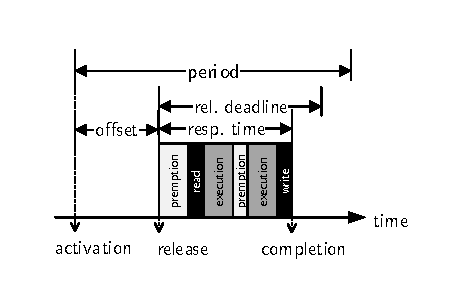
\includegraphics[trim=0.5cm 0.5cm 0.5cm 0.5cm, width=\textwidth]{fig/paper/model_task.pdf}
	\caption{Periodic BET task with release offset.}
	\label{fig:et_task}
\end{subfigure}
%
\hfill
%
\begin{subfigure}[t]{0.45\textwidth}
	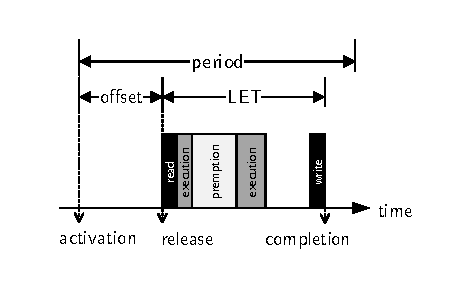
\includegraphics[trim=0.5cm 0.5cm 0.5cm 0.5cm, width=\textwidth]{fig/paper/model_task_let.pdf}
	\caption{LET task with release offset.}
	\label{fig:let_task}
\end{subfigure}
%
\caption{Task model.}
\label{fig:task}
\end{figure}


An \emph{application} is a directed graph $\app = (\taskSet, \dependSet)$, where the set of vertices $\taskSet$ represents the tasks in the application and the set of directed edges $\dependSet$ represents the data-flow dependencies among the tasks. 
An exemplary application is shown in Figure \ref{fig:model_applications}.
\bigskip

\begin{definition}[Cause-effect chain]
A cause-effect chain  
$\cec=(\task[1], \task[2], \ldots, \task[n])$ 
is a finite directed walk in an application $\app$ which is executed on a hardware platform $\platform$.
\end{definition}

\begin{definition}[Instance of a cause-effect chain]
An instance of a cause-effect chain $\cec(\jobSeq)$ 
is a sequence of jobs
$\left(\job[1][j_1], \job[2][j_2], \ldots, \job[n][j_n]\right)$, where each job $\job[{k+1}][j_{k+1}]$ reads data from the predecessor job $\job[k][j_{k}]$.
\end{definition}
%
The concepts of a cause-effect chain and an instance of a cause-effect chain are illustrated in Figure \ref{fig:cec}.
The possible instances of a cause-effect chain can be determined by a data flow analysis, which checks whether a data flow through the sequence of jobs $\job[1][j_1] \job[2][j_2], \ldots, \job[n][j_n]$ is at all possible. 
Please refer to the appendix for details how to perform such a data flow analysis.
\bigskip

The tool \Tool supports time-triggered and LET-triggered cause-effect chains, i.e., cause-effect chains with consists either of only BET tasks or LET tasks.

\begin{figure}
%
\begin{subfigure}[b]{0.5\textwidth}
	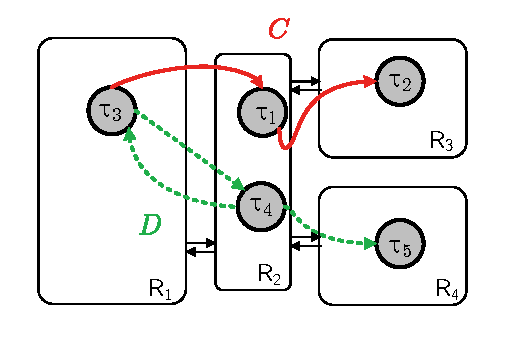
\includegraphics[trim=0.5cm 0.5cm 0.5cm 0.5cm, width=\textwidth]{fig/paper/model_application.pdf}
	\caption{Exemplary cause-effect chains\\ 
	$\cec=(\task[1], \task[2], \task[3])
	= (\taskStd[3], \taskStd[1], \taskStd[2])$  
	and\\ 
	$D=(\task[1][D], \task[2][D], \task[3][D],\task[4][D],\task[5][D])
	= (\taskStd[3], \taskStd[4], \taskStd[3], \taskStd[4], \taskStd[5])$\\
	in an application.}
	\label{fig:model_applications}	
\end{subfigure}
%
\hfill
%
\begin{subfigure}[b]{0.45\textwidth}
	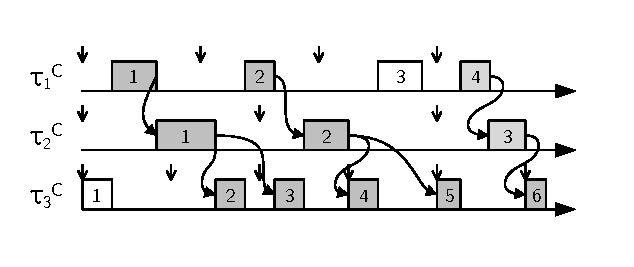
\includegraphics[trim=0.5cm 0.5cm 0.5cm 0.5cm, width=\textwidth]{fig/paper/model_cec_inst.pdf}
	\caption{Exemplary instances of a cause-effect chain  
	$\cec=(\task[\cec_1], \task[2], \task[3])$: \\ 
	$\cec(1,1,2)= \left(\job[1][1], \job[2][1], \job[3][2]\right)$ \\
	$\cec(1,1,3)= \left(\job[1][1], \job[2][1], \job[3][3]\right)$ \\	
	$\cec(2,2,4)= \left(\job[1][2], \job[2][2], \job[3][4]\right)$ \\	
	$\cec(2,2,5)= \left(\job[1][2], \job[2][2], \job[3][5]\right)$ \\	
	$\cec(4,3,6)= \left(\job[1][4], \job[2][3], \job[3][6]\right)$ 
	}
	\label{fig:model_cec}	
\end{subfigure}
%
\caption{Modeling cause-effect chains.}
\label{fig:cec}
\end{figure}

\newpage
\subsubsection{Exemplary Analyzable Systems}
\label{sec:system-model-examples}

\textbf{Application on a single-core ECU} under the following assumptions
\begin{itemize}
	\item Only time-triggered xor LET-triggered cause-effect chains.
	\item Each task meets its deadline or LET.
\end{itemize}

\textbf{Application on a multi-core ECU} under the following assumptions
\begin{itemize}
	\item Only time-triggered xor LET-triggered cause-effect chains.
	\item Each task meets its deadline or LET.
	\item All cores have a common clock, all schedules start simultaneously.
\end{itemize}
%
\textbf{Distributed application on a systems with multiple ECUS connected by data buses and networks} under the following assumptions
	\begin{itemize}
	\item Only time-triggered xor LET-triggered cause-effect chains. 
	\emph{Note that messages can also be modeled as tasks.}
	\item Each task meets its deadline or LET.
	\item All clocks are synchronized, all schedules start simultaneously.
\end{itemize} 
	
\newpage
\subsection{Latencies and Robustness Margins}
\label{sec:outputs}
This section describes which system properties are computed by \Tool. 
For details \emph{how} these properties are computed, please refer to the appendix.


\subsubsection{Maximum End-to-End Latencies}
There are different definitions for end-to-end latencies of cause-effect chains.  
Each definition is relevant in specific contexts, but the most important one is the following:
%
\begin{definition}[End-to-end latency, also: data age]
The end-to-end latency  of an instance of a cause-effect chain, denoted as $\lat{\cec(\jobSeq)}$, is the maximum amount of time that may elapse from the release of the first job $\job[1][j_1]$ to the completion of the last job~$\job[n][j_n]$ in~$\cec(\jobSeq)$.
\end{definition}
%
\begin{definition}[Maximum end-to-end latency]
The maximum end-to-end latency $\latMax$ of a cause-effect chain $\cec$ is an upper bound on the end-to-end latency of any of its instances
\begin{align*}
	\latMax =
	\max_{\cec(\jobSeq) \in \mathcal{C}} 
	\left\{ 
	\lat{\cec(\jobSeq)} 
	\right\}.
\end{align*}
\end{definition}

The maximum end-to-end latency describes how long it can take until fresh input data at the beginning of the cause-effect chain (e.g. a sensor sample) impacts the output of a cause-effect chain (e.g. actuator control value).
This property is important for the reactivity of the system and practical timing requirements often do not  relate to the deadline of tasks but in particular to end-to-end deadlines. 
Tasks deadlines are auxiliary values which emerge in the course of design and implementation.
%
\begin{definition}[End-to-end deadline]
An end-to-end deadline $\eteDeadline$ is the maximum tolerable end-to-end latency of a cause-effect chain $\cec$.
\end{definition}
%


\subsubsection{Robustness Margins}
\label{sec:robustness-margins}
While the maximum end-to-end latency of a cause-effect chain is an important property of the present design, robustness margins indicate to what degree the tasks in a cause-effect chain can be extended in terms of their worst-case response time, resp. LET, without violating timing constraints. 
\bigskip

The tool \Tool computes four different types of robustness margins
\begin{itemize}
	\item Robustness margins for an isolated cause-effect chain  which guarantees the end-to-end deadline
	\item Robustness margins for an isolated cause-effect chain  which guarantees the end-to-end deadline \emph{and} all task deadlines
	\item Robustness margins for a set of possibly dependent cause-effect chains which guarantees all end-to-end deadlines,
	\item Robustness margins for a set of possibly dependent cause-effect chains which guarantees all end-to-end deadlines \emph{and} all task deadlines.			
\end{itemize}
The last type of robustness margin is probably the most important one in practice.


\paragraph{Robustness Margins For an Isolated Cause-Effect Chain} 
This section states the meaning of robustness margins for an isolated cause-effect chain. 
The theorems are based on the paper in the appendix.

\begin{tcolorbox}[colback=black!5!white,colframe=black!75!black, breakable, 
title= \textbf{Theorem}: Robustness test for a single time-triggered cause-effect chain]
Let $\cec = (\task[1], \task[2], \ldots, \task[n])$ be a time-triggered cause-effect chain with the property that each task $\task[k]$ in $\cec$ has a worst-case response time $\wcrt{k}$ satisfying the task deadline $\deadline{k}$. 
Moreover, the cause-effect chain $\cec$ also satisfies its end-to-end deadline $\eteDeadline$.
Let $\disturb[k] \geq 0$ be the increase in the worst-case response time of each task $\task[k]$ in $\cec$ that is caused by a software update.
\smallskip

The time-triggered cause-effect chain $\cec$ still satisfies its end-to-end deadline $\eteDeadline$ under the increase of the worst-case response times of its tasks $\task[k]$ by $\disturb[k]$, if  
\begin{align*}
	& \forall \task[k] \in \cec: \:
	\disturb[k] < \margin{\task[k]} .
\end{align*}	

The time-triggered cause-effect chain $\cec$ still satisfies its end-to-end deadline $\eteDeadline$ \emph{and its task deadlines} under the increase of the worst-case response times of its tasks $\task[k]$ by $\disturb[k]$, if  
\begin{align*}
	& \forall \task[k] \in \cec: \:
	\disturb[k] < 
	\min \{\margin{\task[k]}, \: \deadline{k} - \wcrt{k}\}.
\end{align*}	

\end{tcolorbox}
\smallskip

\begin{tcolorbox}[colback=black!5!white,colframe=black!75!black, breakable, 
title= \textbf{Theorem}: Robustness test for a single LET-triggered cause-effect chain]
Let $\cec = (\task[1], \task[2], \ldots, \task[n])$ be a LET-triggered cause-effect chain with the property that each task $\task[k]$ in $\cec$ satisfies its LET $\Let{k}$. 
Moreover, the cause-effect chain $\cec$ also satisfies its end-to-end deadline $\eteDeadline$.
Let $\disturbLet{k} \geq 0$ be a planned increase of the $\Let{k}$ of a task $\task[k]$.
\smallskip

The LET-triggered cause-effect chain $\cec$ still satisfies its end-to-end deadline $\eteDeadline$ under the increase of the LETs of its tasks $\task[k]$ by $\disturbLet{k}$, if  
\begin{align*}
	& \forall \task[k] \in \cec: \:
	\disturbLet{k} < \margin{\task[k]}. 
\end{align*}	

The LET-triggered cause-effect chain $\cec$ still satisfies its end-to-end deadline $\eteDeadline$ \emph{and its task deadlines} under the increase of the worst-case response times of its tasks $\task[k]$ by $\disturb[k]$, if  
\begin{align*}
	& \forall \task[k] \in \cec: \:
	\disturb[k] < 
	\min \{\margin{\task[k]}, \: \deadline{k} - \Let{k}\}.
\end{align*}	

\end{tcolorbox}
\bigskip

\newpage
\paragraph{Robustness Margins for a Set of Possibly Dependent Cause-Effect Chains}
A task of an application may be part of several cause-effect chains.
Consequently, increasing the worst-case response time (or LET) of this particular task may have an impact on all cause-effect chains that share this task.
We can find new robustness margins $\marginAll{\task[k]}$ (instead of: $\margin{\task[k]}$) which guarantee that \emph{all} cause-effect chains in the application still satisfy their deadlines under a disturbance $\disturb[k]$ resp. $\disturbLet{k}$.
\bigskip

\begin{tcolorbox}[colback=black!5!white,colframe=black!75!black, breakable, 
title= \textbf{Theorem} (Robustness test for time-triggered cause-effect chains)]
Let $\mathcal{S}$ be a set of time-triggered cause-effect chains. 
Each cause-effect chain $\cec = (\task[1], \task[2], \ldots, \task[n])$ in $\mathcal{S}$ has the property that the worst-case response time $\wcrt{k}$ of every task $\task[k]$ in $\cec$ satisfies the task deadline $\deadline{k}$. 
Moreover, each cause-effect chain $\cec$ in $\mathcal{S}$ also satisfies its end-to-end deadline $\eteDeadline$.
%
Let $\disturb[k] \geq 0$ be the increase in the worst-case response time of a task $\task[k]$ in $\taskSet$ that is caused by a software update.
\smallskip

All time-triggered cause-effect chain $\cec$ in $\mathcal{S}$ still satisfy their end-to-end deadlines $\eteDeadline$ under the increase of the worst-case response times of its tasks $\task[k]$ by $\disturb[k]$, if  
\begin{align*}
	& \forall \cec: \forall \task[k] \in \cec: \:
	\disturb[k] < \marginAll{\task[k]}. 
\end{align*}	

All time-triggered cause-effect chain $\cec$ in $\mathcal{S}$ still satisfy their end-to-end deadlines $\eteDeadline$ \emph{and all task deadlines} under the increase of the worst-case response times of its tasks $\task[k]$ by $\disturbLet{k}$, if  
\begin{align*}
	& \forall \task[k] \in \cec: \:
	\disturb[k] < 
	\min \{\marginAll{\task[k]}, \: \deadline{k} - \wcrt{k}\}.
\end{align*}

\end{tcolorbox}
\bigskip

\begin{tcolorbox}[colback=black!5!white,colframe=black!75!black, breakable, 
title= \textbf{Theorem} (Robustness test for LET-triggered cause-effect chains)]
Let $\mathcal{S}$ be a set of LET-triggered cause-effect chains. 
Each cause-effect chain $\cec = (\task[1], \task[2], \ldots, \task[n])$ in $\mathcal{S}$ has the property that every task $\task[k]$ in $\cec$ satisfies its LET $\Let{k}$. 
Moreover, each cause-effect chain $\cec$ in $\mathcal{S}$ also satisfies its end-to-end deadline $\eteDeadline$.
%
Let $\disturbLet{k} \geq 0$ be a planned increase of the $\Let{k}$ of a task $\task[k]$.
\smallskip

All LET-triggered cause-effect chain $\cec$ in $\mathcal{S}$ still satisfy their end-to-end deadlines $\eteDeadline$ under the increase of the LETs of its tasks $\task[k]$ by $\disturbLet{k}$, if  
\begin{align*}
	& \forall \cec: \forall \task[k] \in \cec: \:
	\disturbLet{k} < \marginAll{\task[k]}. 
\end{align*}	

All LET-triggered cause-effect chain $\cec$ in $\mathcal{S}$ still satisfy their end-to-end deadlines $\eteDeadline$ \emph{and all task deadlines} under the increase of the LETs of its tasks $\task[k]$ by $\disturbLet{k}$, if  
\begin{align*}
	& \forall \task[k] \in \cec: \:
	\disturb[k] < 
	\min \{\marginAll{\task[k]}, \: \deadline{k} - \Let{k}\}.
\end{align*}	

\end{tcolorbox}







